
Le module de raisonnement est subdivisé en deux sous modules : le \og moteur de choix \fg{} chargé de la prise de décision et le \og moteur d'introspection \fg{} chargé d'extraire de nouvelles formes remarquables.
Le moteur de choix est chargé de la partie  prise de décision du module  de raisonnement pour ce faire celui-ci sera \og stimulé \fg{} par le module d'analyse lorsque un ensemble de plateau est disponible en mémoire. Le moteur de choix doit être capable de choisir, de façon rationnel, un plateau parmi l'ensemble proposé. Pour cela, notre IA se base sur la valuation des formes remarquables (représentées sous la forme d'une formule de logique du première ordre) associées à  nos  états de plateaux possibles. En fin de partie, elle met en œuvre un mécanisme permettant la mise à jour de la valuation des différentes \og configurations \fg{} rencontrées au cours de celle-ci en fonction du résultat final de la partie.
Le moteur d'introspection est chargé de la  partie réorganisation et évaluation des \og concepts \fg{} rencontrés. Il  examine à posteriori les raisons d'une victoire où d'une défaite grâce à  la mémoire épisodique pour optimiser ses chances de victoire futur. {+ découverte nouveaux RPBS}

Le module de raisonnement est subdivisé en deux sous modules. Le premier appelé \og moteur de choix \fg{} doit être capable de choisir, de façon rationnel, un environnement parmi un ensemble proposé. Le second appelé \og raisonneur \fg{} doit être capable de trouver de nouvelles formes remarquables à partir d'une analyse de ses diverses expériences passées.

\subsubsection{Raisonneur}

Le module de raisonnement a pour objectif d'extraire, à partir des expériences passées de l'IA, de nouvelles formes remarquables potentiellement discriminante pour les choix futurs. Pour ce faire, il choisi aléatoirement, en mémoire, au moins deux environnements ayant reçu la même annotations et tente d'étendre les formes déjà reconnues.

\begin{figure}[H] 
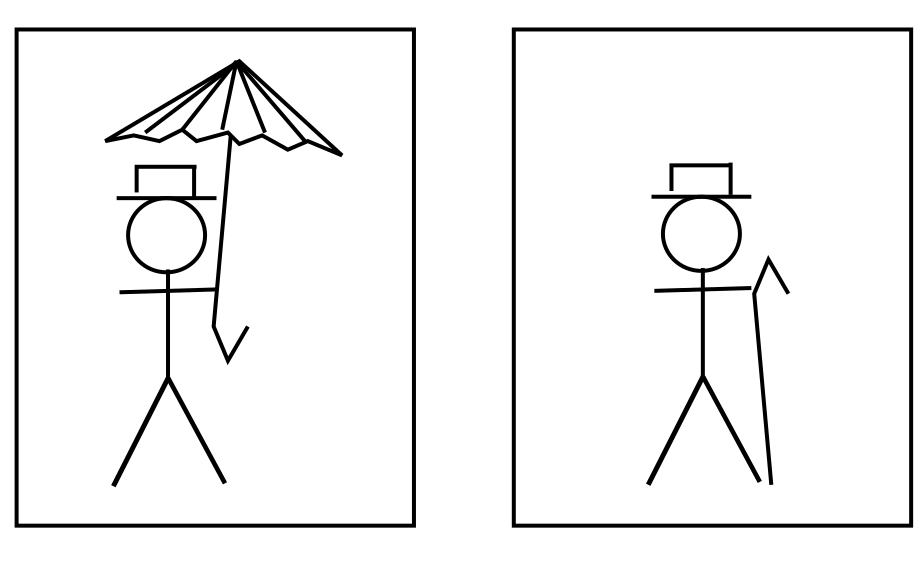
\includegraphics[width=\textwidth]{files/raisonneur/reconnaissance_de_formes_0} 
\caption{Illustration de la reconnaissance de forme 0} 
\end{figure}

\subsubsection{Moteur de choix}

Ce module intervient après la phase d'analyse qui lui fourni, par l'intermédiaire de la mémoire, un ensemble d'environnements possibles et pour chacun un ensemble de formes reconnues. Le \og moteur de choix \fg{} se sert alors de la valuation des formes remarquables (valuation effectuer précédemment) pour évaluer chaque environnement possible. Il choisi finalement l'environnement qui maximise la fonction objectif.



